\begin{figure}
\centering
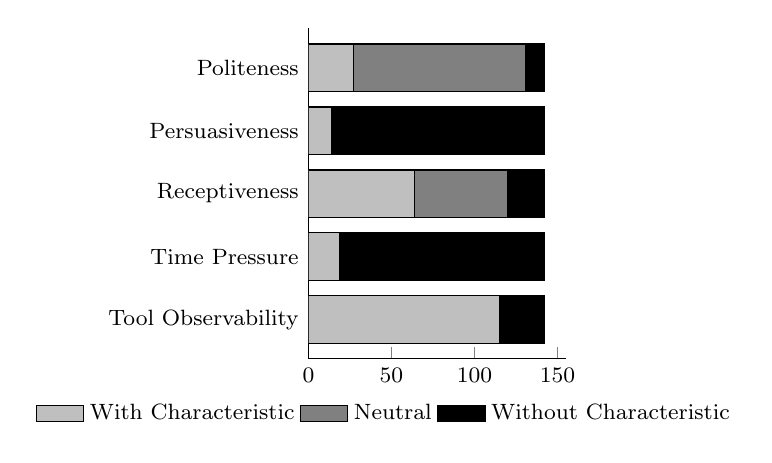
\begin{tikzpicture}
\begin{axis}[
    xbar stacked,
    legend style={
    legend columns=3,
        at={(xticklabel cs:0.3)},
        anchor=north,
        draw=none
    },
    ytick=data,
    axis y line*=none,
    axis x line*=bottom,
    tick label style={font=\footnotesize},
    legend style={font=\footnotesize},
    label style={font=\footnotesize},
    xtick={0,50,100,150},
    width=.4\textwidth,
    bar width=6mm,
    xlabel= Number of Recommendations,
    yticklabels={Tool Observability, Time Pressure, Receptiveness, Persuasiveness, Politeness},
    xmin=0,
    xmax=155,
    area legend,
    y=8mm,
    enlarge y limits={abs=0.625},
]
% With
\addplot[fill=lightgray] coordinates
{(115,0) (19,1) (64,2) (14,3) (27,4)};
% Neutral
\addplot[fill=gray] coordinates
{(0,0) (0,1) (56,2) (0,3) (104,4)};
% Without
\addplot[fill=black] coordinates
{(27,0) (123,1) (22,2) (128,3) (11,4)};
\legend{With Characteristic, Neutral, Without Characteristic}
\end{axis}  
\end{tikzpicture}
\caption{Peer Interaction Characteristic Results}
\label{fig:peer-chars}
\end{figure}